% --------------------------------------------------------------
% This is all preamble stuff that you don't have to worry about.
% Head down to where it says "Start here"
% --------------------------------------------------------------
 
\documentclass[12pt]{article}

\usepackage{courier}
\usepackage{color}
\usepackage{listings}
\usepackage[square,numbers]{natbib}
\usepackage{tabls}
\usepackage{graphicx}
\usepackage{subcaption}
\usepackage{pdfpages}
\usepackage{mathtools}

\definecolor{dkgreen}{rgb}{0,0.6,0}
\definecolor{gray}{rgb}{0.5,0.5,0.5}




\lstset{language=python,
   basicstyle=\ttfamily,
   keywordstyle=\color{blue},
   commentstyle=\color{dkgreen},
   stringstyle=\color{red},
   numbers=left,
   numberstyle=\tiny\color{gray},
   stepnumber=1,
   numbersep=10pt,
   backgroundcolor=\color{white},
   tabsize=4,
   showspaces=false,
   showstringspaces=false}
 
\usepackage[margin=1in]{geometry} 
\usepackage{amsmath,amsthm,amssymb}
\usepackage{verbatim}
\usepackage{algpseudocode,algorithm}
\usepackage{setspace}

\newcommand{\ihat}{\ensuremath{\hat{\textbf{\i}}}}
\newcommand{\jhat}{\ensuremath{\hat{\textbf{\j}}}}
\newcommand{\lline}{\noindent\makebox[\linewidth]{\rule{\textwidth}{0.4pt}}}
\newcommand{\N}{\mathbb{N}}
\newcommand{\Z}{\mathbb{Z}}
\newcommand{\deriv}[2]{\frac{\mathrm{d} #1}{\mathrm{d} #2}}
\newcommand{\pderiv}[2]{\frac{\partial #1}{\partial #2}}
\newcommand{\bx}{\mathbf{X}}
\newcommand{\ba}{\mathbf{A}}
\renewcommand{\d}{\mathrm{d}}
\newcommand{\A}{\frac{(1-\alpha)}{2(1+\alpha)}}
\newcommand{\upl}{u_{\text{plane}}}
\newcommand{\upt}{u_{\text{point}}}
\newcommand{\D}{\Delta}
\newcommand{\ra}{\rightarrow}
\renewcommand{\SS}{\State}
 
\newenvironment{theorem}[2][Theorem]{\begin{trivlist}
\item[\hskip \labelsep {\bfseries #1}\hskip \labelsep {\bfseries #2.}]}{\end{trivlist}}
\newenvironment{lemma}[2][Lemma]{\begin{trivlist}
\item[\hskip \labelsep {\bfseries #1}\hskip \labelsep {\bfseries #2.}]}{\end{trivlist}}
\newenvironment{exercise}[2][Exercise]{\begin{trivlist}
\item[\hskip \labelsep {\bfseries #1}\hskip \labelsep {\bfseries #2.}]}{\end{trivlist}}
\newenvironment{problem}[2][Problem]{\begin{trivlist}
\item[\hskip \labelsep {\bfseries #1}\hskip \labelsep {\bfseries #2:}]\hspace{0.3in}\newline\newline}{\end{trivlist}}
\newenvironment{question}[2][Question]{\begin{trivlist}
\item[\hskip \labelsep {\bfseries #1}\hskip \labelsep {\bfseries #2.}]}{\end{trivlist}}
\newenvironment{corollary}[2][Corollary]{\begin{trivlist}
\item[\hskip \labelsep {\bfseries #1}\hskip \labelsep {\bfseries #2.} ]}{\end{trivlist}}
\newenvironment{problem*}[1][Problem]{\begin{trivlist}
\item[\hskip \labelsep {\bfseries #1} {\hspace{-0.2em}\bfseries:}]}{\end{trivlist}}
\newenvironment{solution}[1][Solution]{\begin{trivlist}
\item[\hskip \labelsep {\bfseries #1} {\hspace{-0.2em}\bfseries:}]\hspace{0.3in}\newline}{\end{trivlist}}
 
\begin{document}
 
% --------------------------------------------------------------
%                         Start here
% --------------------------------------------------------------
 
\title{Homework 2}%replace X with the appropriate number
\author{Simon Bolding\\ %replace with your name
NUEN 629} %if necessary, replace with your course title
 
\maketitle

\clearpage

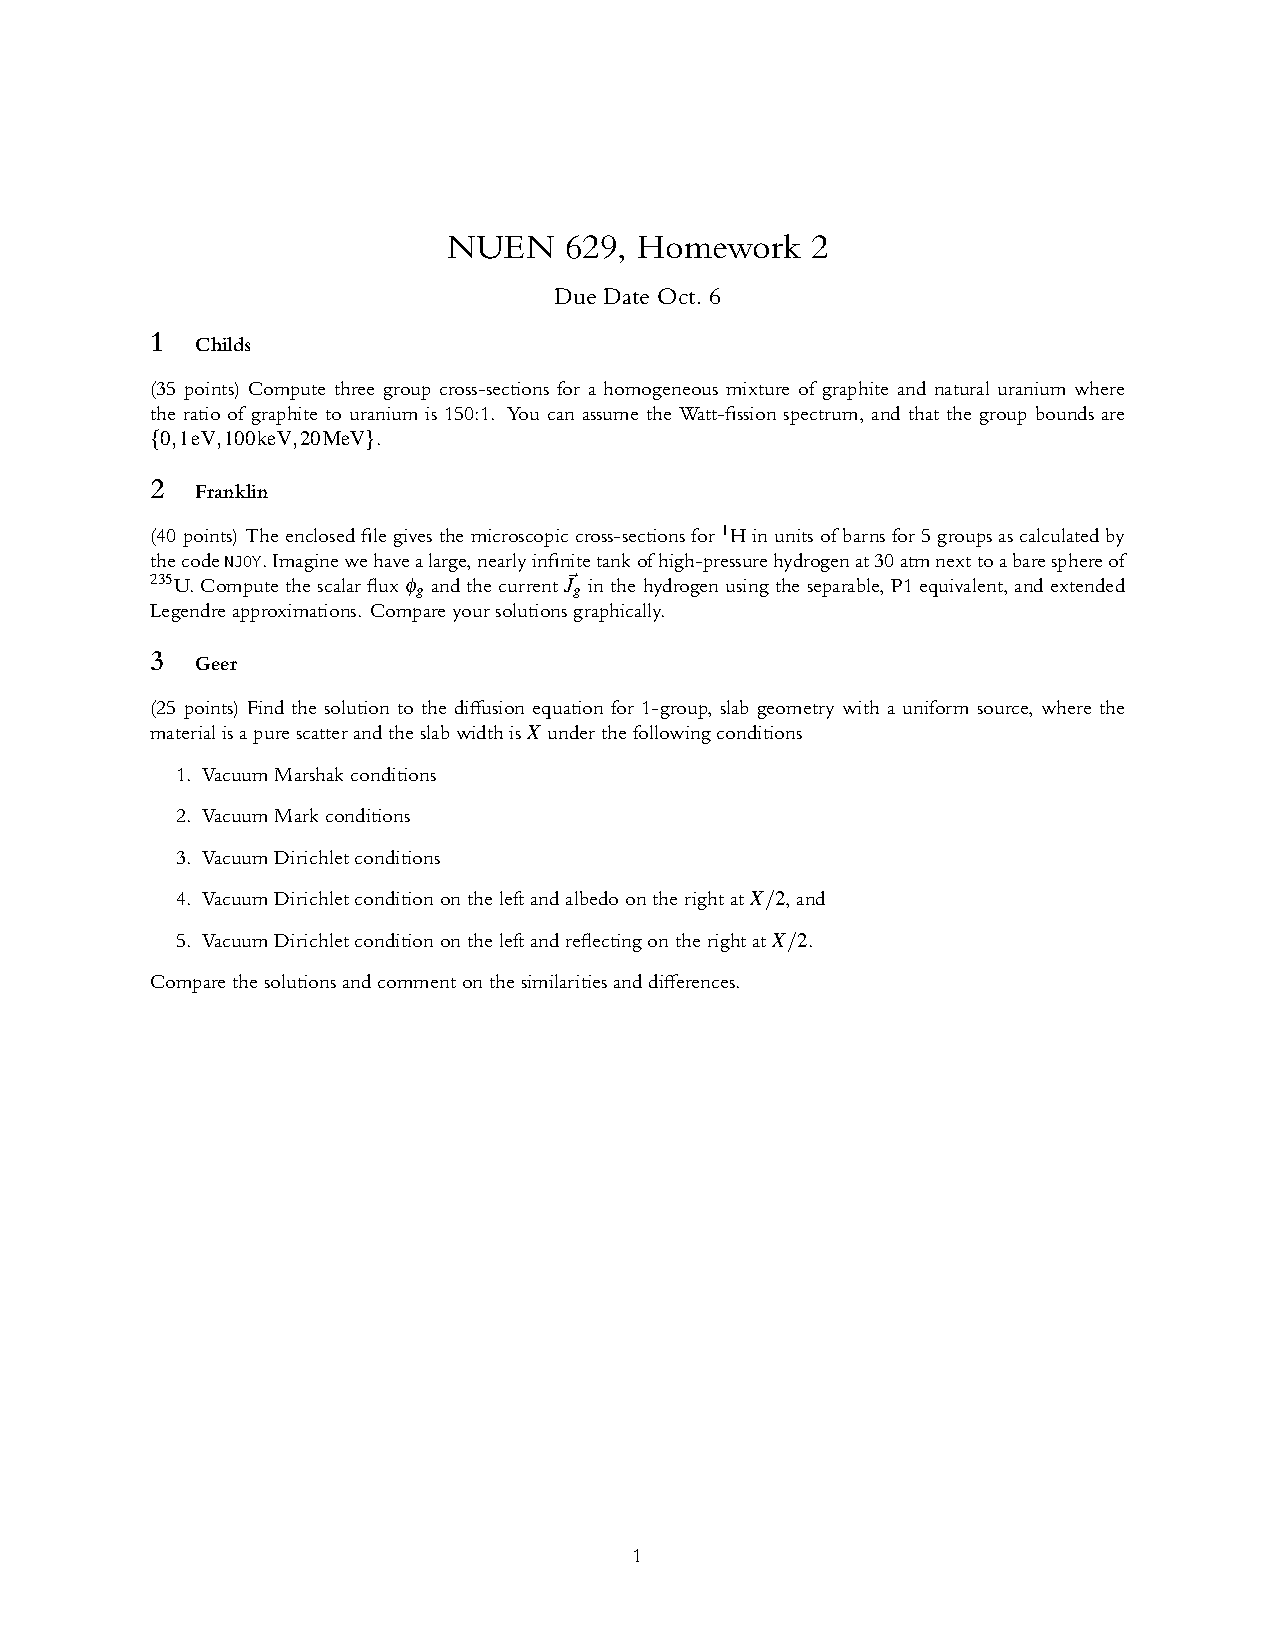
\includepdf{Homework2.pdf}

%\includepdf[pages={1}]{p1p3.pdf}
\clearpage
    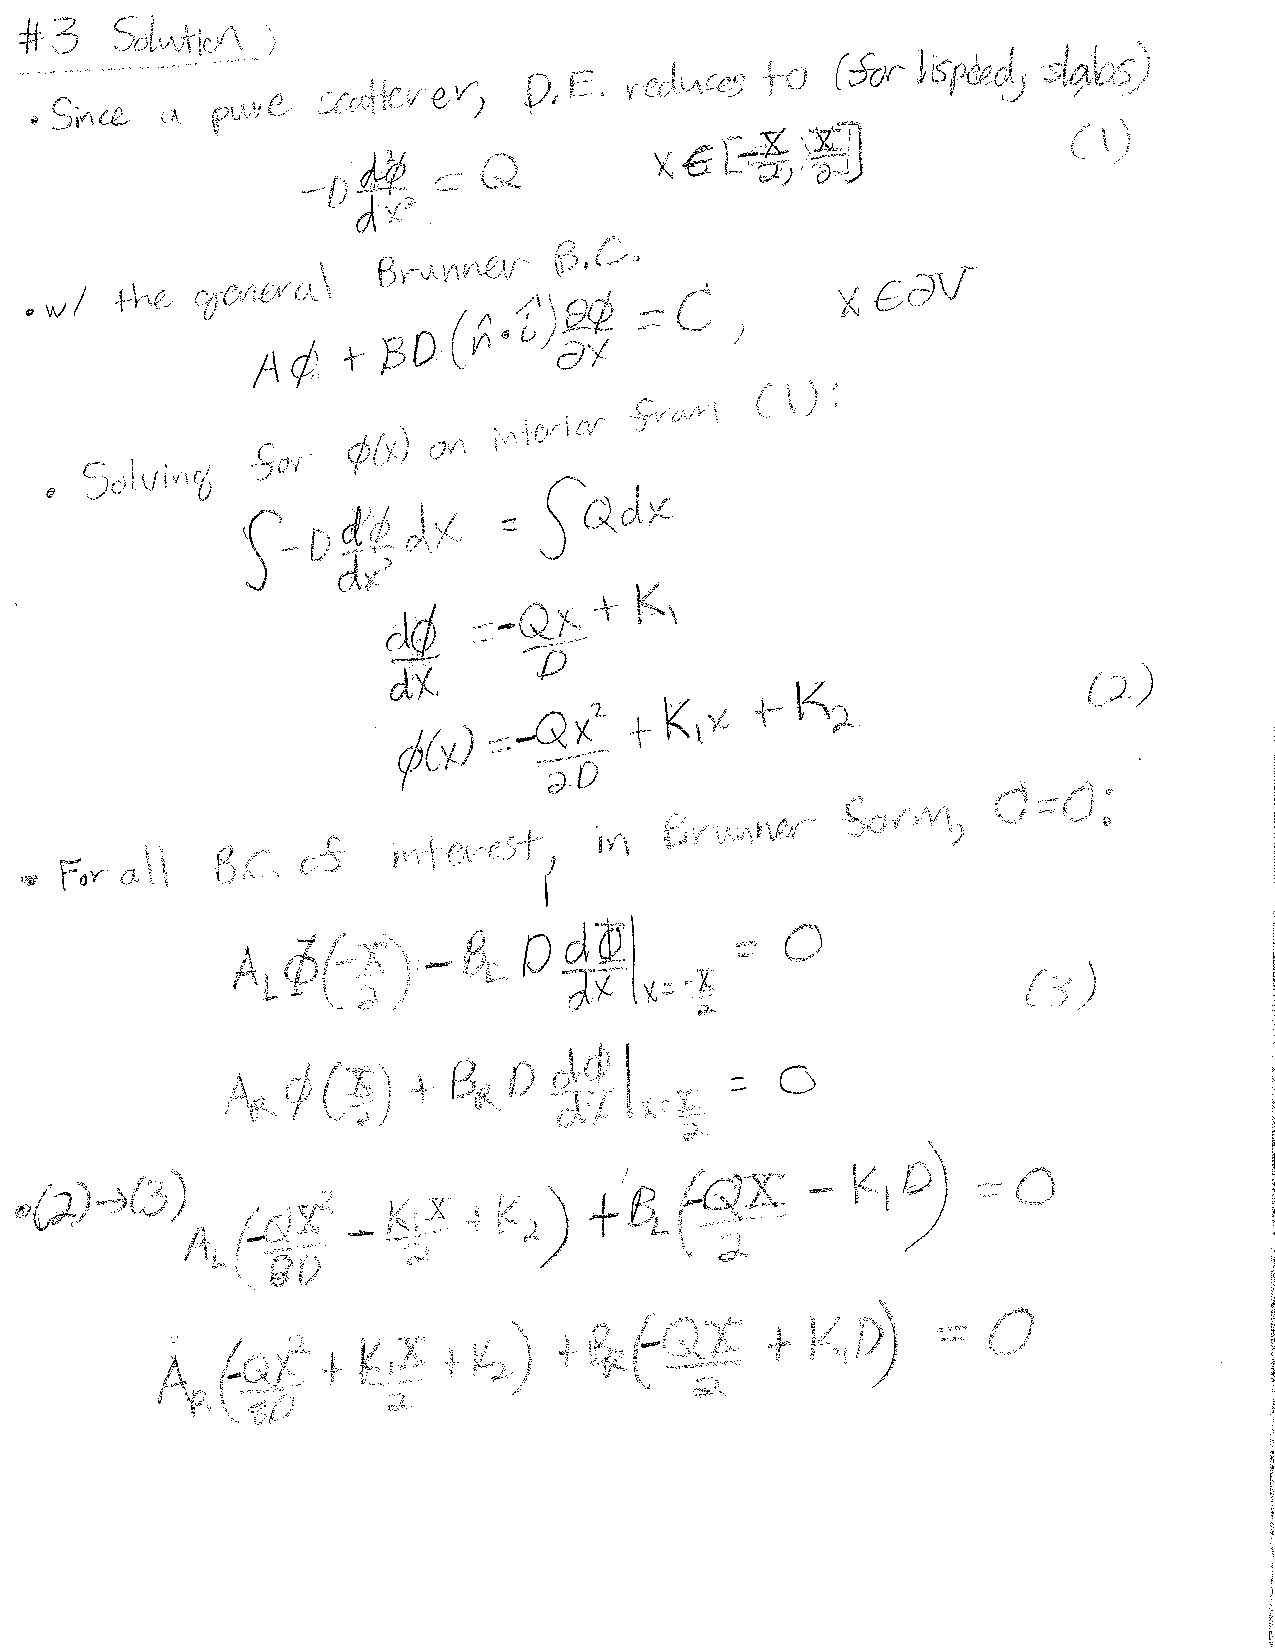
\includepdf[pages={1-2}]{p3.pdf}
    A summary of the solutions obtained for each of the boundary conditions is given
    in the table below.  Each solution was checked to ensure they satisfy the
    boundary conditions.
    \begin{table}[h]
        \centering
        \caption{Solutions with different boundary conditions for  a pure scatter for slab of width $X$ centered at
        $x=0$.}
        \begin{tabular}{|c|c|c|} \hline
            Left BC & Right BC & $\phi(x)$ \\ \hline
            Vacuum Marshak & Vacuum Marshak & $\phi(x) = Q\left(\frac{X^2}{8D} + X-\frac{x^2}{2D} 
            \right)            $ \\ 
            Vacuum Mark & Vacuum Marshak & $\phi(x) = Q\left(
            \frac{X^2}{8D} + \frac{X\sqrt{3}}{2}-\frac{x^2}{2D}\right)$ \\ 
            Vacuum Dirichlet  & Vacuum Dirichlet & $\phi(x) = \frac{Q}{2D}\left( 
            \frac{X^2}{4} - x^2\right)  $ \\ 
            Vacuum Dirichlet    & Albedo  & $\phi(x) = -\frac{Qx^2}{2D} +
            QxX\left(\frac{1+\A\frac{X}{2D}}{\A X + D} - \frac{1}{2D}  \right) +
            Q\frac{X^2}{2} \left(\frac{1+\A\frac{X}{2D}}{\A X +
            D}-\frac{1}{4D}\right) $ \\
            Vacuum Dirichlet    & Reflecting & $\phi(x) =
            \frac{Q}{2D}\left(\frac{3X^2}{4} + xX  - {x^2}\right)$ \\ \hline
        \end{tabular}
    \end{table}
\clearpage


\end{document}

